\documentclass[12pt]{article}
\usepackage{graphicx} % Required for inserting images
\graphicspath{{./images/}}
\usepackage[margin=2cm]{geometry}
\usepackage{booktabs}
\usepackage{adjustbox}

\usepackage{hyperref}
\urlstyle{same}

\usepackage{amsmath}
\usepackage{amssymb}

\title{}
\author{}
\date{}

\begin{document}

% --------------
%  Requirements 
% --------------

% Main objective of the analysis that also specifies whether your model will be focused on clustering or dimensionality reduction and the benefits that your analysis brings to the business or stakeholders of this data.

% Brief description of the data set you chose, a summary of its attributes, and an outline of what you are trying to accomplish with this analysis.

% Brief summary of data exploration and actions taken for data cleaning orfeature engineering.

% Summary of training at least three variations of the unsupervised model you selected. For example, you can use different clustering techniques or different hyperparameters.

% A paragraph explaining which of your Unsupervised Learning models you recommend as a final model that best fits your needs in terms.

% Summary Key Findings and Insights, which walks your reader through the main findings of your modeling exercise.

% Suggestions for next steps in analyzing this data, which may include suggesting revisiting this model or adding specific data features to achieve a better model.

\section*{Introduction}

% Main objective of the analysis that also specifies whether your model will be focused on clustering or dimensionality reduction and the benefits that your analysis brings to the business or stakeholders of this data.

Customer classification is a common practice for targeted advertising which leverages purchase history and demographic information to deliver new deals and advertisements to those who are most likely to engage with them. In addition to the benefits brought to the customers, this method can also significantly cut advertising costs by limiting their scope while also identifying those areas where deals and discounts would be the most effective. Here, we will focus on clustering in order to partition a specific customer base into a few basic groups. 

% Brief description of the data set you chose, a summary of its attributes, and an outline of what you are trying to accomplish with this analysis.

The data set used here contains 2240 samples of customer data which contain various kinds of information about their spending habits as well as demographic information which may influence those habits. The included features can broadly be split into personal information, purchase history, and engagement. These groups and the features associated with them are summarized below. This data can be found on Kaggle at \url{https://www.kaggle.com/datasets/imakash3011/customer-personality-analysis/data}.
\vspace{1em}

\begin{tabular}{l l p{4in}}
    \toprule
    Group & Type & Features \\
    \midrule
    Personal & Numeric & Year\_Birth, Income, Kidhome (number of children), Teenhome (number of teens), Dt\_Customer (date enrolled), Recency (days since last purchase) \\
     & Categorical & Education, Marital\_Status, Complain (if customer complained in last 2 years) \\
    \\
    Purchase History & Numeric & MntWines, MntFruits, MntMeatProducts, MntFishProducts, MntSweetProducts, MntGoldProds (amount spent on a product) \\
    \\
    Engagement & Numeric & NumWebPurchase (number of purchase on website), NumCatalogPurchases, NumStorePurchases, NumWebVisitsMonth (number of website visits in last month) \\
     & Categorical & NumDealsPurchases (number of purchase with discount), AccpetedCmp1 (if accepted offer from campaign 1), AcceptedCmp2, AcceptedCmp3, AcceptedCmp4, AcceptedCmp5, Response (if accepted offer in last campaign) \\
    \bottomrule
\end{tabular}
\vspace{1em}

With this data set, we will cluster the data into a small number of customer profiles. Several different clustering algorithms with various hyperparameters will be used to determine a few basic clusters and cross-referenced with one another to ensure they are not outliers. Once the customers are partitioned into groups we can compare the means of each cluster to determine what kind of consumer demographic they represent.

\section*{Exploratory Data Analysis}

% Brief summary of data exploration and actions taken for data cleaning orfeature engineering.

The full data set contains 2240 samples, however several samples contain null values for their income. After removing those samples, we are left with 2216 samples. Before we can scale the numerical data, the feature Dt\_Customer first needs to be transformed from a string into a number of days. Using numpy's \texttt{to\_datetime()} function, the strings are transformed into Python's \texttt{datetime} format. From here, the minimum date is subtracted from the column, setting the minimum to 0, and then the values are replaced with only the number of days from the resulting \texttt{timedelta} object. Several of the numeric features, especially Income and the amounts spent on different products have skew values greater than 1, so a log transformation is applied to features with a skew greater than 0.7. Each of the numeric features are then scaled using standard scaling. Finally, the categorical features of Education and Marital\_Status are encoded. 

From the correlation matrix of the features, we can already begin to see some patterns. Below is a subsection of the correlation matrix which shows the greatest feature correlations. One of the main insights here is that the amount of money spent in all categories is positively correlated to the customer's income. Similarly, other than the number of purchases made with a deal, all purchase types are positively correlated to income. As one might expect, having more money lets you make more purchases. 
\begin{center}
    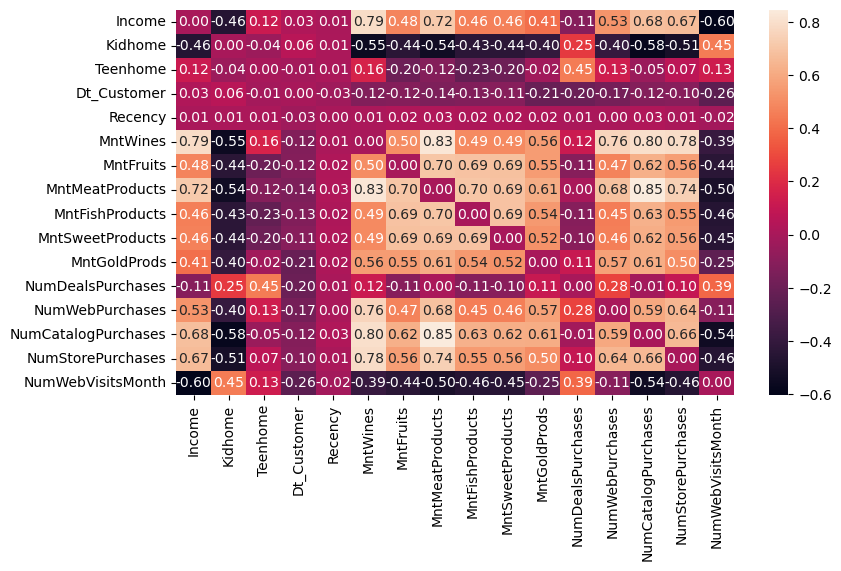
\includegraphics[width=6.5in]{images/corr_mat.png}
\end{center}

\section*{Model Training}

% Summary of training at least three variations of the unsupervised model you selected. For example, you can use different clustering techniques or different hyperparameters.

Three clustering models were used to partition the data set, and each had hyperparameters tuned to give comparable results. These models are K-means, hierarchical agglomerate clustering, and mean shift. DBSCAN was not used, as the data doesn't form any distinct clusters, so the algorithm cannot find any clusters and labels all data as outliers unless a significantly large epsilon value is given. Even then, the largest cluster corresponds to $\sim90\%$ of the data and the other clusters are essentially just small clusters of similar outliers. From the pairplot of the scaled data (present in the appendix), it is easy to see that much of the data is overlapping, and assignment via DBSCAN would be difficult.

For the K-means model, we first examined the inertia as the number of clusters changed. As seen on the graph, there is not an obvious elbow point, so we investigated the classes individually. 
\begin{center}
    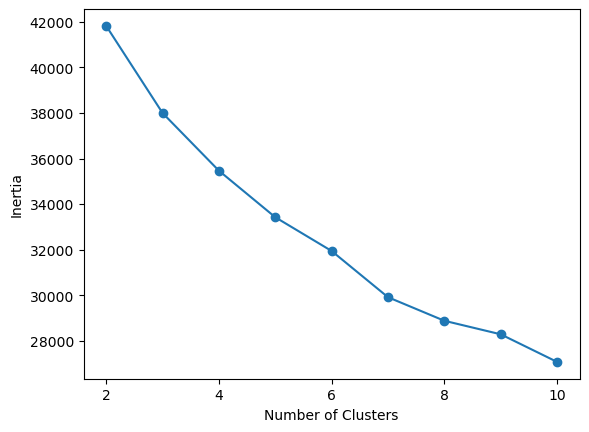
\includegraphics[width=4in]{images/inertia.png}
\end{center}
The ideal number of clusters was decided to be 3, as splitting further to 4 clusters seemed to mostly divided a larger cluster unnecessarily. With 3 clusters, the main feature that separates them is once again Income. With more Income, a customer can spend more and that is reflected in the amounts spent on each of the goods. 
\begin{center}
    \begin{tabular}{lrrrrrrr}
    \toprule
    Cluster &   Income &  Wines &  Fruits &  Meat &  Fish &  Sweets &  Gold \\
    \midrule
    0 & 75573.27 &    607.44 &      64.47 &           438.02 &            96.96 &             66.78 &         76.04 \\
    1 & 33045.70 &     27.46 &       3.80 &            19.79 &             5.29 &              4.20 &         12.48 \\
    2 & 56820.03 &    397.47 &      23.66 &           132.69 &            30.28 &             23.43 &         56.10 \\
    \bottomrule
    \end{tabular}
\end{center}
However, there are other trends that can be observed in the clusters. On average, the customers with higher incomes had fewer children, and the middle income group had more teens than young children. This aligns well with the trend that the middle income customers were also on average older than the lower income customers by a few years. We can likely assume that they have been working longer and their children are older. 
\begin{center}
    \begin{tabular}{lrrrr}
    \toprule
    Cluster &   Income &  Year\_Birth &  Kidhome &  Teenhome \\
    \midrule
    0 & 75573.27 &     1968.41 &     0.03 &      0.14 \\
    1 & 33045.70 &     1972.02 &     0.82 &      0.42 \\
    2 & 56820.03 &     1965.45 &     0.31 &      0.88 \\
    \bottomrule
    \end{tabular}
\end{center}
Finally, we can also see trends in their spending habits. The high income customers make the largest number of purchases, and all three groups make the largest number of purchases in-store. The information could help decided where to or where not to focus advertising. Cluster 1 in the largest, but don't make web purchases often, so trying to advertise to them there would not be effective. There is also information on the advertising campaigns that each cluster did or did not respond to, but it is hard to draw any meaningful conclusions as the data does contain any further details about those campaigns. 
\begin{center}
    \begin{tabular}{lccccccccc}
    \toprule
    Center &  Deals &  Web &  Catalog &  Store &  Cmp1 &  Cmp2 &  Cmp3 &  Cmp4 &  Cmp5 \\
    \midrule
    0 &               1.12 &             5.05 &                 5.80 &               8.33 &          0.21 &          0.04 &          0.09 &          0.14 &          0.27 \\
    1 &               1.89 &             1.85 &                 0.45 &               2.94 &          0.00 &          0.00 &          0.07 &          0.01 &          0.00 \\
    2 &               3.73 &             5.93 &                 2.87 &               7.19 &          0.02 &          0.01 &          0.07 &          0.10 &          0.01 \\
    \bottomrule
    \end{tabular}
\end{center}
The K-means model with 4 clusters splits off a small portion of the high income customers into a higher income category, with similar statistics, but boosted to spend more money and make more purchases. It seems reasonable to stay with 3 clusters, as this distinction is likely minor in regards to targeted advertising.

Hierarchical agglomerate clustering gives similar results to the K-means model. The means of the clusters and the conclusions that can be drawn from them are the same, with the minor difference that more of the samples are shifted into lower income clusters, i.e. fewer high and middle income customers and more low income customers. The mean shift model gives similar clusters as well, but finds that only 30 customers are in the high income cluster and 21 are in the low, with the remaining 2165 in the middle. This model is much more sensitive to the tight proximity of the clusters, and these 3 clusters were only achievable with a bandwith of 8. With a bandwidth of 7, the mean shift algorithm finds 9 different clusters. 

% A paragraph explaining which of your Unsupervised Learning models you recommend as a final model that best fits your needs in terms.

Based on these results, the hierarchical agglomerate cluster model would be recommended. The mean shift model heavily favors the average of the entire data set and does not respond will to the tight clustering. While both the K-means and hierarchical agglomerate clustering models gave similar results, the K-means model still contains a random element which could more easily be affected by outliers. We would also expect that the low income customers would be the largest group, and thus would  lead to an imbalance in the cluster density and further distort the K-means results. 

\section*{Summary}

% Summary Key Findings and Insights, which walks your reader through the main findings of your modeling exercise.

This data set presented here was analyzed using different clustering algorithms. Both the K-means and hierarchical agglomerate clustering algorithms found 3 clusters which primarily corresponded to high, middle, and low income customers. This was the largest determining factor in how much a customer spent on any given product type. These clusters engaged with the company in a variety of ways, but they mostly preferred to make their purchases in-store, though the customers with more income were more likely to order from catalogs or from the website, methods which often cost extra due to shipping and delivery costs. These results can be used to focus advertising efforts, such as tailoring website adds to the high and middle income earners who are more likely to order from the website. There is also information on which groups engaged with various advertising campaigns, but it is difficult to draw any conclusions without more information on those specific campaigns. The hierarchical agglomerate clustering model provides the best performance while also being less affected by the unbalanced class distribution. 

% Suggestions for next steps in analyzing this data, which may include suggesting revisiting this model or adding specific data features to achieve a better model.

To improve this analysis, it would be useful to create more separable clusters. The clusters found here are relatively close to each other, making some clustering methods like mean shift impractical to use. This could be accomplished by finding more features which have greater variance and would further split the clusters, or eliminating some of the unnecessary features with dimensionality reduction. 

\newpage

\section*{Appendix}
\small
Compiled means for each model

\begin{center}    
\begin{adjustbox}{angle=90}
    \begin{tabular}{lccccccccc}
    \toprule
    {} & \multicolumn{3}{c}{K-means} & \multicolumn{3}{c}{Hierarchical Agglomerate} & \multicolumn{3}{c}{Mean Shift} \\
    Feature &        0 &        1 &        2 &           0 &        1 &        2 &          0 &        1 &        2 \\
    \midrule
    Size                &   574 &   879 &   763 &      535 &  1057 &   624 &    2165 &    30 &    21 \\
    Year\_Birth          &  1968.41 &  1972.02 &  1965.45 &     1967.99 &  1971.00 &  1965.85 &    1968.87 &  1968.13 &  1965.10 \\
    Income              & 75573.27 & 33045.70 & 56820.03 &    74858.95 & 36828.27 & 58978.99 &   52054.58 & 71054.83 & 45242.29 \\
    Kidhome             &     0.03 &     0.82 &     0.31 &        0.04 &     0.74 &     0.27 &       0.44 &     0.07 &     0.67 \\
    Teenhome            &     0.14 &     0.42 &     0.88 &        0.14 &     0.46 &     0.89 &       0.51 &     0.43 &     0.52 \\
    Recency             &    49.56 &    48.08 &    49.67 &       48.37 &    48.38 &    50.63 &      48.98 &    48.67 &    53.05 \\
    MntWines            &   607.44 &    27.46 &   397.47 &      620.78 &    79.16 &   417.14 &     298.19 &   898.67 &   169.00 \\
    MntFruits           &    64.47 &     3.80 &    23.66 &       59.80 &     7.09 &    30.31 &      26.42 &    22.97 &    24.19 \\
    MntMeatProducts     &   438.02 &    19.79 &   132.69 &      432.27 &    37.84 &   158.32 &     166.37 &   250.30 &   112.48 \\
    MntFishProducts     &    96.96 &     5.29 &    30.28 &       89.49 &     9.81 &    40.32 &      37.74 &    38.73 &    25.76 \\
    MntSweetProducts    &    66.78 &     4.20 &    23.43 &       61.28 &     6.89 &    31.78 &      27.07 &    30.60 &    17.52 \\
    MntGoldProds        &    76.04 &    12.48 &    56.10 &       72.67 &    20.76 &    58.66 &      43.81 &    66.40 &    27.48 \\
    NumDealsPurchases   &     1.12 &     1.89 &     3.73 &        1.31 &     2.09 &     3.59 &       2.33 &     1.70 &     2.33 \\
    NumWebPurchases     &     5.05 &     1.85 &     5.93 &        5.04 &     2.49 &     5.98 &       4.08 &     4.90 &     3.62 \\
    NumCatalogPurchases &     5.80 &     0.45 &     2.87 &        5.66 &     0.87 &     3.16 &       2.64 &     5.17 &     2.05 \\
    NumStorePurchases   &     8.33 &     2.94 &     7.19 &        8.18 &     3.43 &     7.78 &       5.77 &     8.17 &     5.24 \\
    NumWebVisitsMonth   &     2.76 &     6.53 &     5.85 &        2.99 &     6.43 &     5.44 &       5.32 &     5.17 &     5.81 \\
    AcceptedCmp3        &     0.09 &     0.07 &     0.07 &        0.05 &     0.13 &     0.00 &       0.07 &     0.23 &     0.10 \\
    AcceptedCmp4        &     0.14 &     0.01 &     0.10 &        0.15 &     0.00 &     0.13 &       0.07 &     0.73 &     0.00 \\
    AcceptedCmp5        &     0.27 &     0.00 &     0.01 &        0.29 &     0.01 &     0.00 &       0.07 &     0.57 &     0.05 \\
    AcceptedCmp1        &     0.21 &     0.00 &     0.02 &        0.27 &     0.00 &     0.00 &       0.06 &     0.43 &     0.00 \\
    AcceptedCmp2        &     0.04 &     0.00 &     0.01 &        0.06 &     0.00 &     0.00 &       0.00 &     1.00 &     0.00 \\
    Complain            &     0.01 &     0.01 &     0.01 &        0.00 &     0.02 &     0.00 &       0.00 &     0.00 &     1.00 \\
    Response            &     0.30 &     0.09 &     0.11 &        0.33 &     0.13 &     0.03 &       0.14 &     0.67 &     0.14 \\
    \bottomrule
    \end{tabular}
\end{adjustbox}
\end{center}

\newpage

Subset of a seaborn pairplot using hierarchical agglomerate clusters
\begin{center}
    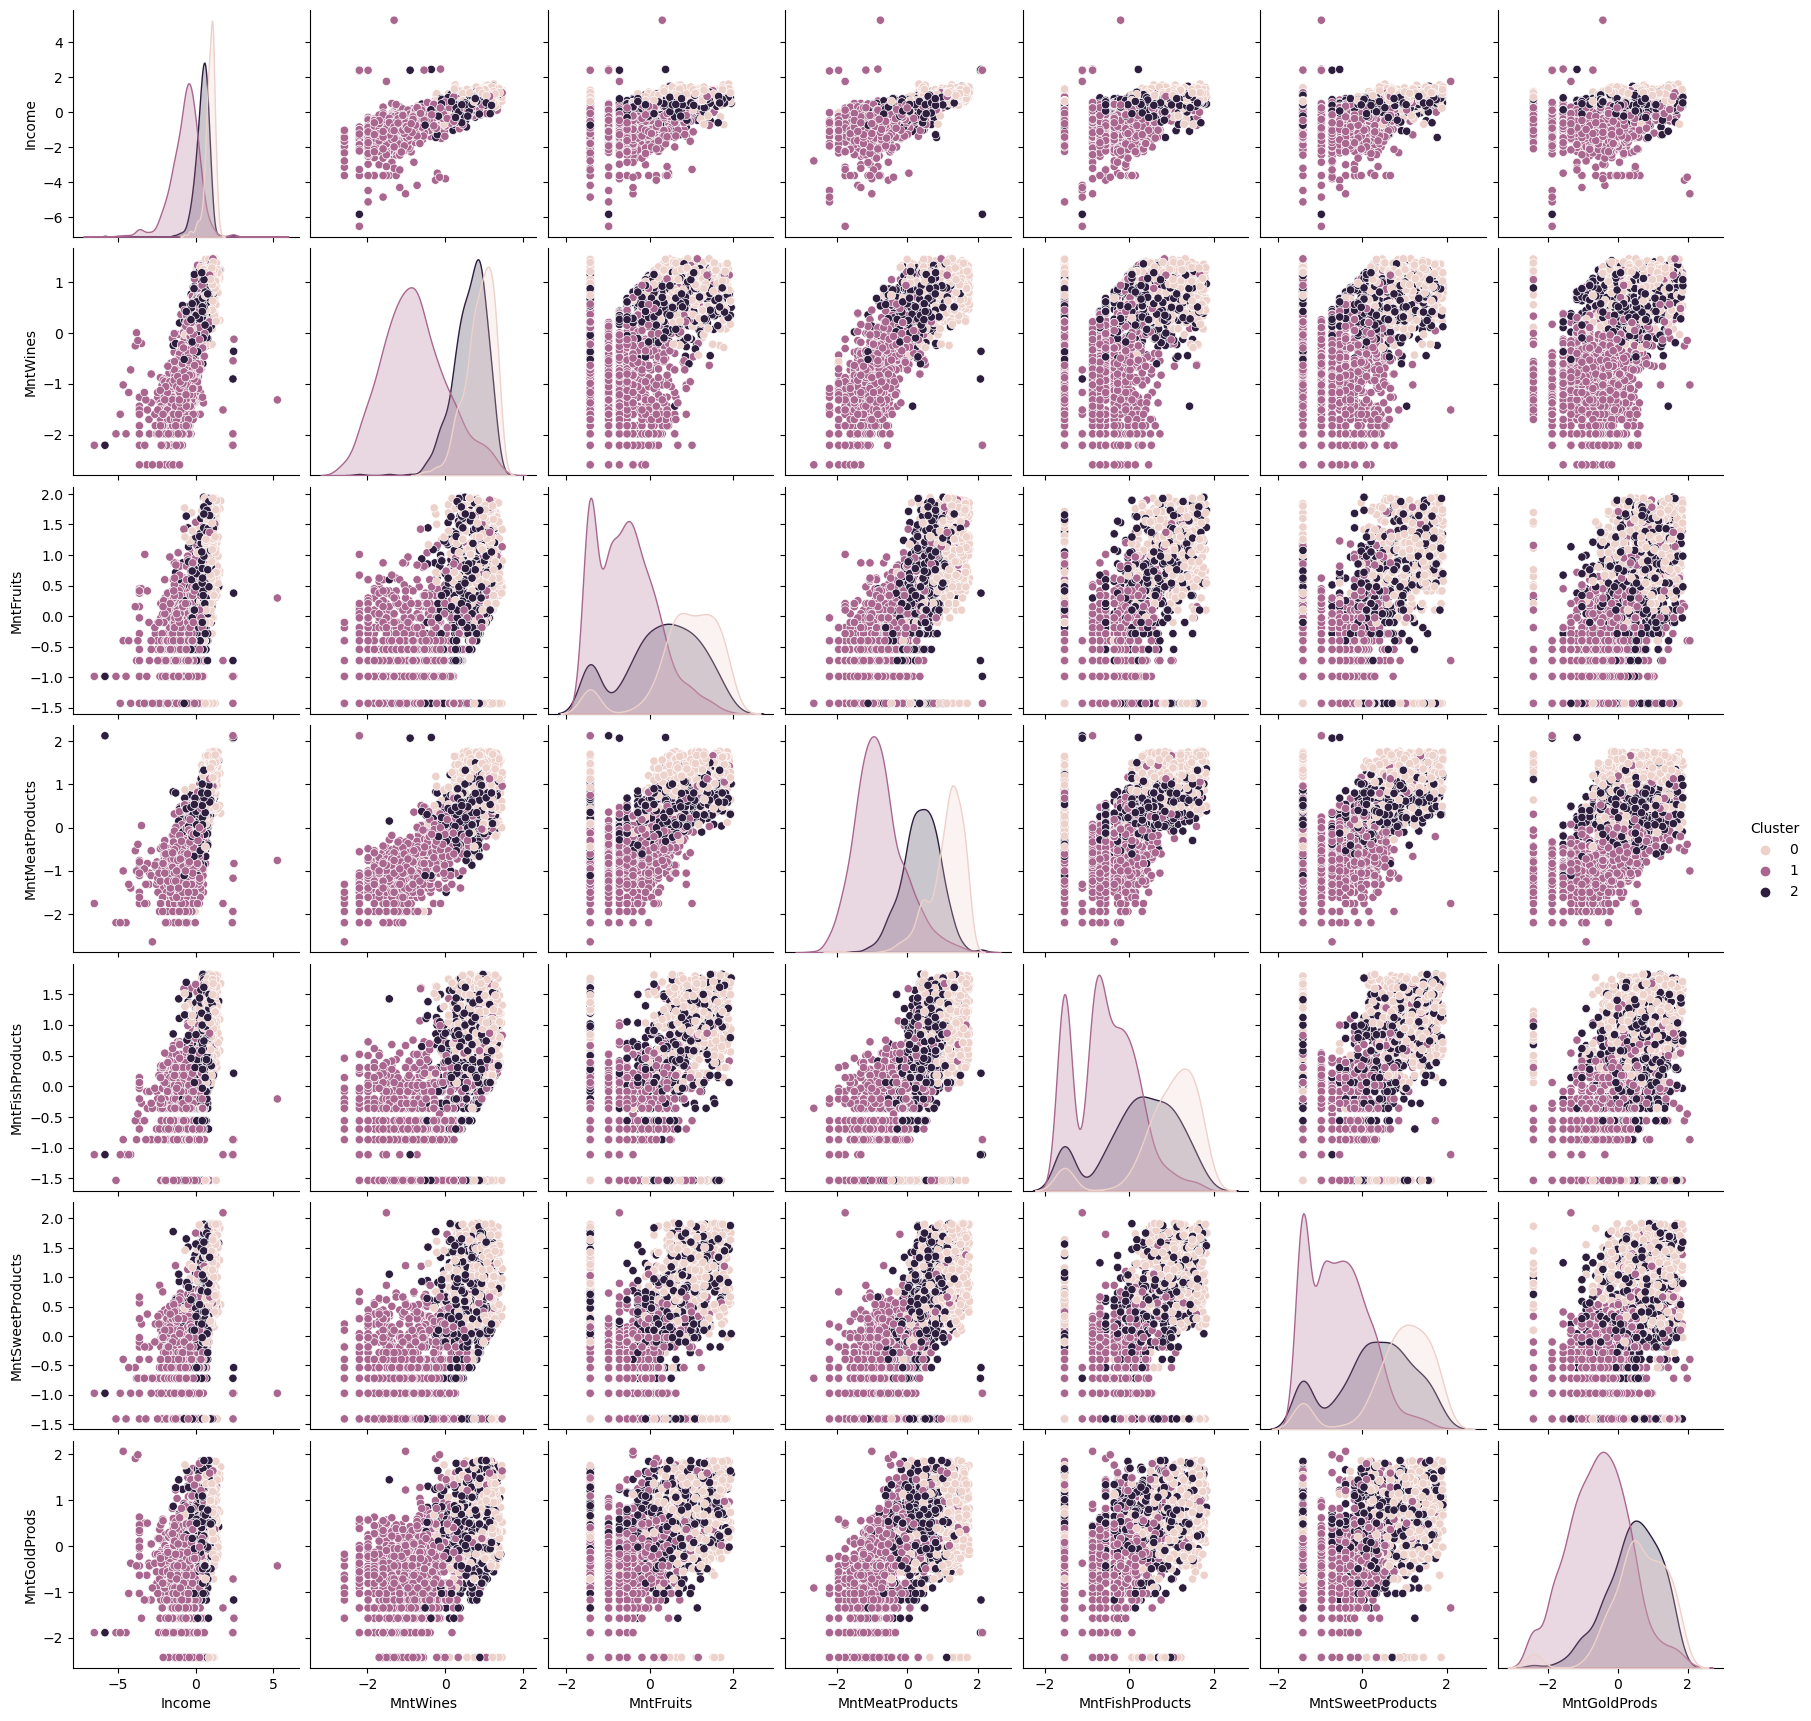
\includegraphics[width=6.5in]{images/pairplot.png}
\end{center}

\end{document}
